\chapter{Concepts}
\label{ch:concepts}
%checked by Bryan @2247, except DOT

In a previous phase of the project, possible concepts were generated after a brainstorm session. Five concepts were chosen to be analysed further in order to obtain one concept that will be a base for a final design \cite{baseline}. The five concepts are briefly described as following:  an airplane-balloon configuration, a tandem wing configuration, a Prandtl boxed wing configuration, a flying ducted wing, and a tiltrotor. Feasibility analysis is carried out based on preliminary calculations to assess feasibility of the five concepts. \autoref{sec:DOT} presents the Design Option Tree (DOT) 
\nomenclature[A]{DOT}{Design Option Tree}
%I rewrote the intro part of this chapter. The original version can be found below. Stephanie, I know that you don't appreciate having things changed without being told, so I am going to leave original paragraphs below edited paragraphs so you can see differences. I am not going to indicate simple word changes though. - Bryan

%In the baseline report, a brainstorm about different possible concepts was presented. After that, five concepts were chosen. These five concepts were to be analysed further, in order to obtain one concept that will be the base for the final design \cite{baseline}. These five concepts were an airplane-balloon configuration, a tandem wing configuration, a Prandtl boxed wing configuration, a flying ducted wing and a concept containing a tilting rotor. Because it was not possible to find any UAVs in the same size range that make use of either a balloon or a duct-mechanism for hovering, it was decided to make some preliminary calculations to ensure feasibility. 

\section{Design Option Tree}
\label{sec:DOT}
%I haven't checked this session - Bryan, 21:48

The Design Option Tree (DOT) can be found in \Cref{fig:DOTmain,fig:DOThover,fig:DOTvto,fig:DOTvl,fig:DOTlift,fig:DOThthrust,fig:DOTstability,fig:DOTprop}. In \autoref{fig:DOTmain}, the main design option tree is presented. This tree starts with the mission need statement and has functions flowing down from it. This tree is an AND-tree since the UAV needs to be able to perform all functions in order to fulfil the mission. The seven different functions are then expanded in OR-trees in \Cref{fig:DOThover,fig:DOTvto,fig:DOTvl,fig:DOTlift,fig:DOThthrust,fig:DOTstability} in order to find design options to fulfil each function. \autoref{fig:DOTprop} depicts the propulsion branch of the tree. This branch is very large and occurs multiple times in the tree, this is why this branch is depicted separately.


\begin{figure}[H]
\centering
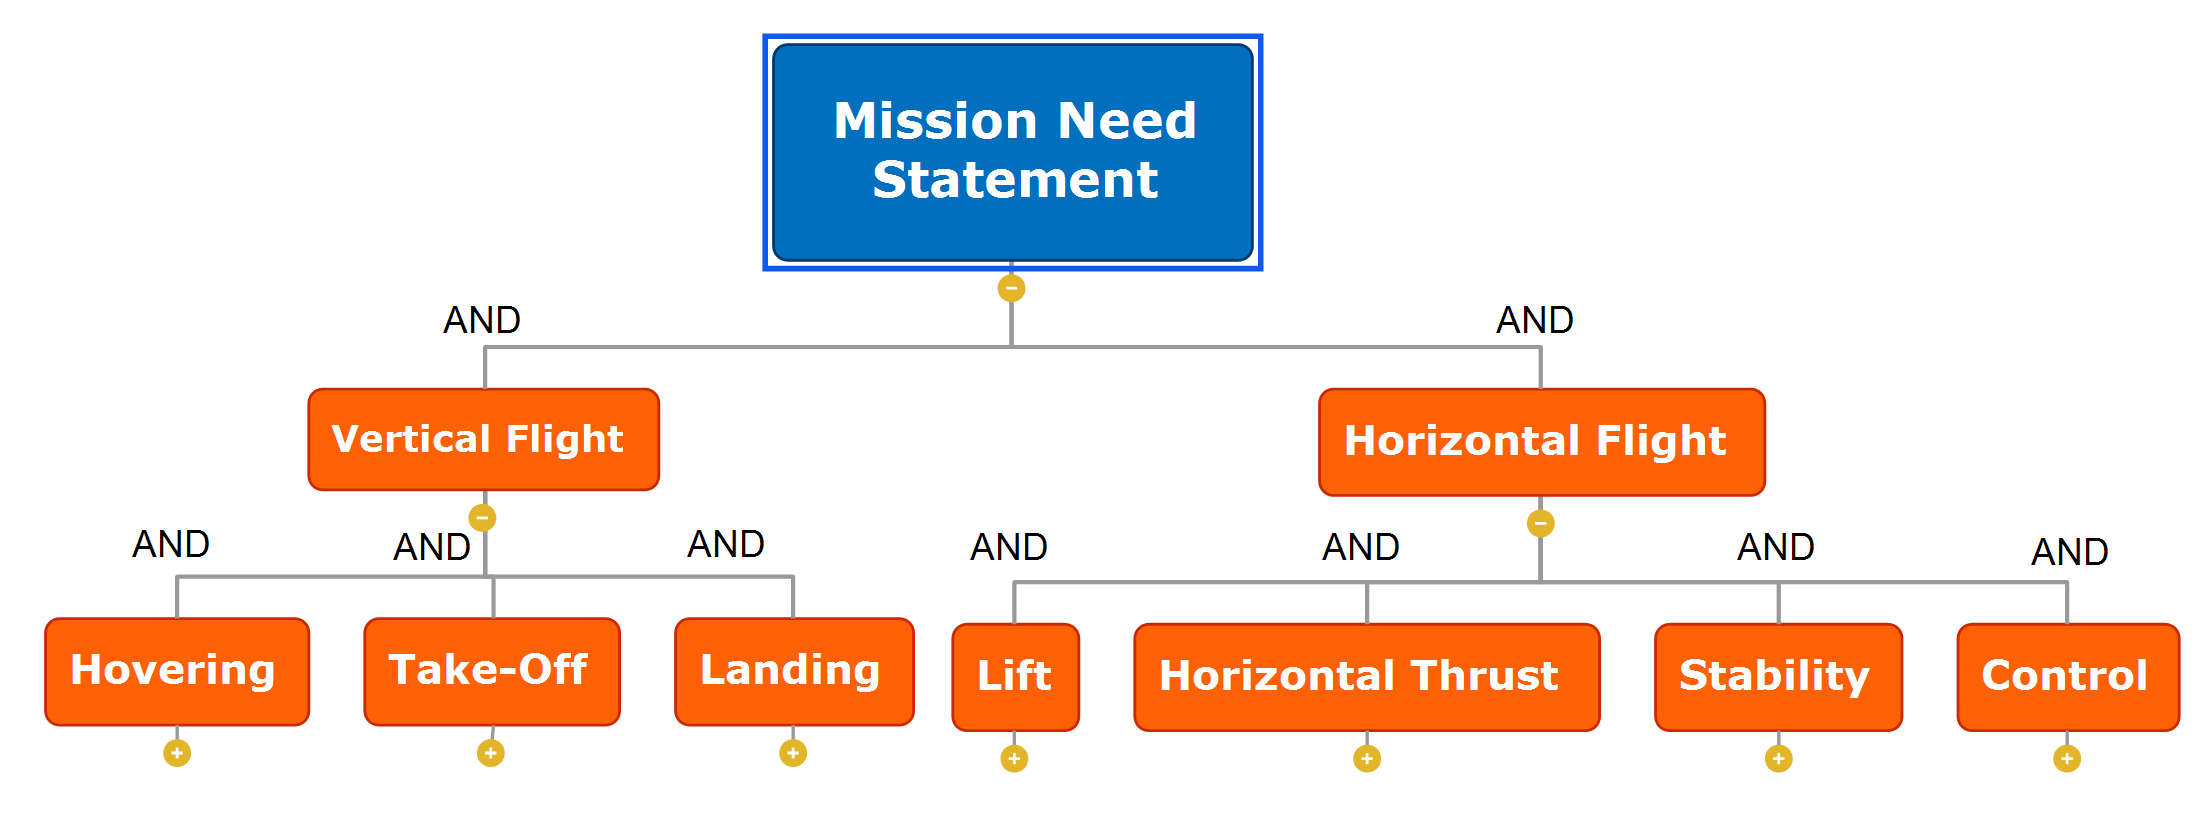
\includegraphics[width=.55\textwidth]{Concepts/Figures/Toplevel}
\caption{Unexpanded design option tree}
\label{fig:DOTmain}
\end{figure}

The first function depicted in the tree is hovering, which is shown in \autoref{fig:DOThover}. This is a major part in various missions, for example monitoring and dropping payload off. There are two branches in the separate hovering tree, propulsion or buoyancy. These two have been chosen by looking at how it is possible to keep an aircraft in the air while stationary. For propulsion there is a whole set of possibilities to get this done, and there are also a lot of possibilities where to get the energy from. This is why this part (under propulsion) is an and-tree. This tree is shown separately in \autoref{fig:DOTprop}. The next part of the branch is buoyancy, which can be achieved with a balloon.

\begin{figure}[H]
\centering
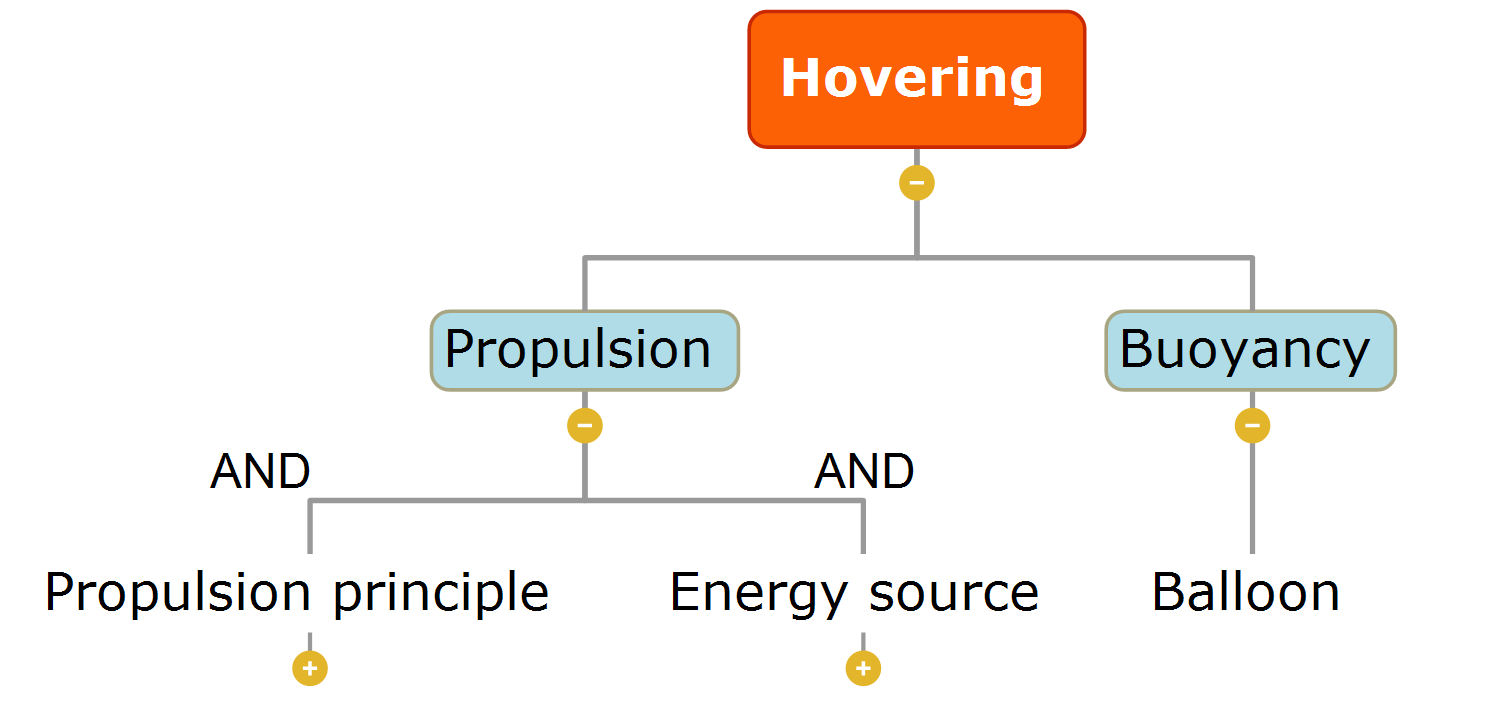
\includegraphics[width=.5\textwidth]{Concepts/Figures/Hovering}
\caption{Hovering branch of the design option tree}
\label{fig:DOThover}
\end{figure}

\autoref{fig:DOTvto} depicts the vertical take-off branch of the design option tree. The vertical take-off functionality is of major importance to the Hybrid UAV design. It allows for operation from almost any location, independent from available ground based infrastructure. This branch is split into three possible means of performing a vertical take-off. These are the light blue coloured blocks on the second level. They are propulsion, buoyancy and kinetic impulse. So, the possibilities are self propelled vertical take-off, lighter than air lift-off or an initial amount of kinetic energy being transferred to the vehicle. The propulsion branch consists of both propulsion principle and energy source. The deeper levels of the propulsion branch of this tree are shown in \autoref{fig:DOTprop} and they will be elaborated on later in this chapter. For buoyancy one can make use of a balloon. For the option of proving an external kinetic impulse to the vehicle there are multiple possibilities. The first method is a sling shot which transfers potential energy from an elastic band to the UAV or a catapult with the similar method. The third method is the trebuchet which transfers gravitational potential energy from a mass to the vehicle.

\begin{figure}[H]
\centering
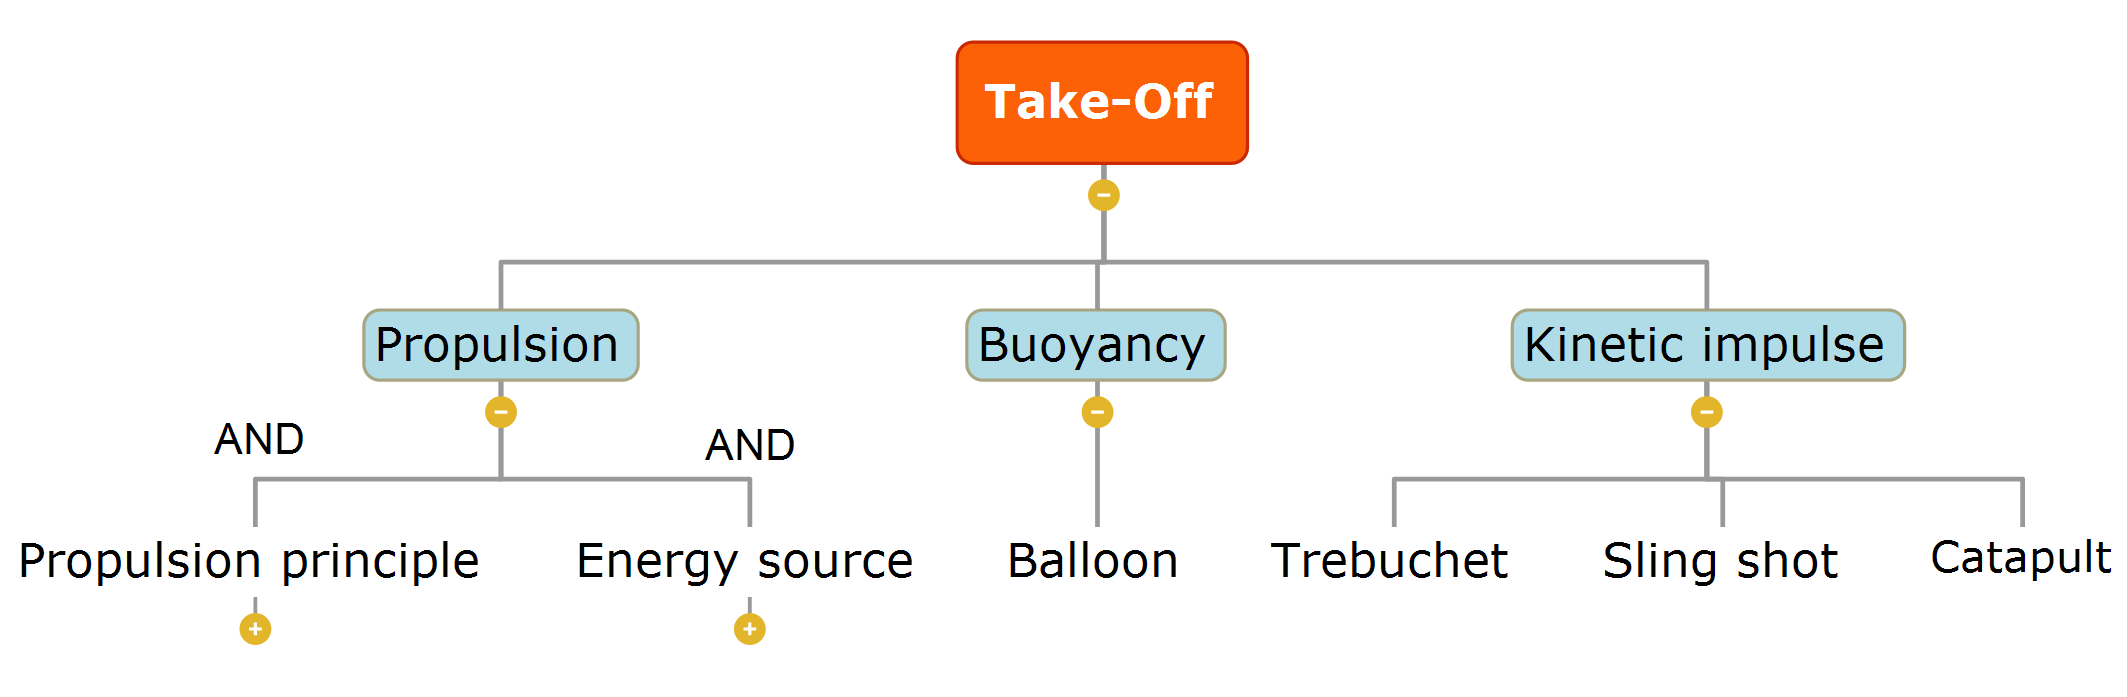
\includegraphics[width=.8\textwidth]{Concepts/Figures/Take-off}
\caption{Vertical take-off branch of the design option tree}
\label{fig:DOTvto}
\end{figure}

The vertical landing capability is a vital element of the Hybrid UAV. It is important for operations on all terrains and reusablity. The vertical landing branch is shown in \autoref{fig:DOTvl}. The propulsive and buoyant options are similar to those in the vertical take-off branch. The option of impact landing is split into three different options. For all of these the vehicle will land vertically with a relatively high velocity and its kinetic energy is absorbed either internally of externally on impact. The impact energy can be absorbed by springs or airbags on the vehicle or by a flexible net on which the UAV will land.

\begin{figure}[H]
\centering
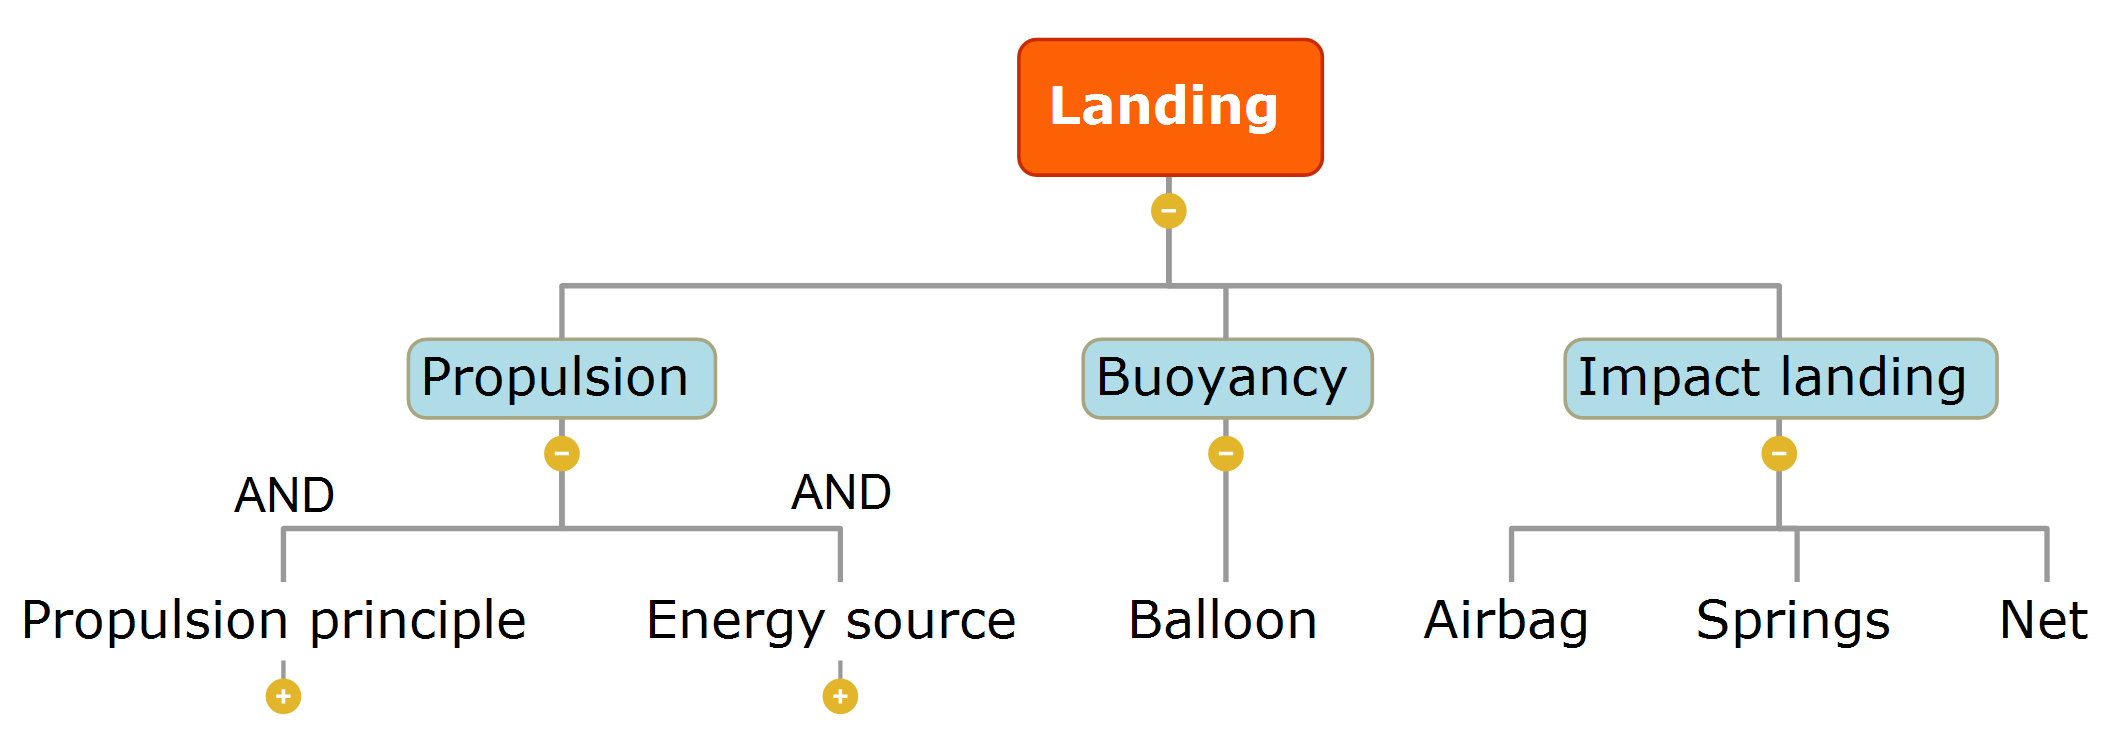
\includegraphics[width=.7\textwidth]{Concepts/Figures/Landing}
\caption{Vertical landing branch of the design option tree}
\label{fig:DOTvl}
\end{figure}

Now that all the functions are done which are connected to VTOL and hovering, it is time to look at how the Hybrid UAV can perform horizontal flight, starting with lift. This branch, shown in \autoref{fig:DOTlift}, is similar to that of the hovering, this is because for hovering you also need to generate some upward force. The main difference here is that you can make use of wings due to the horizontal speed, which is the third branch of this tree. It is possible to have a different amount of wings.

\begin{figure}[H]
\centering
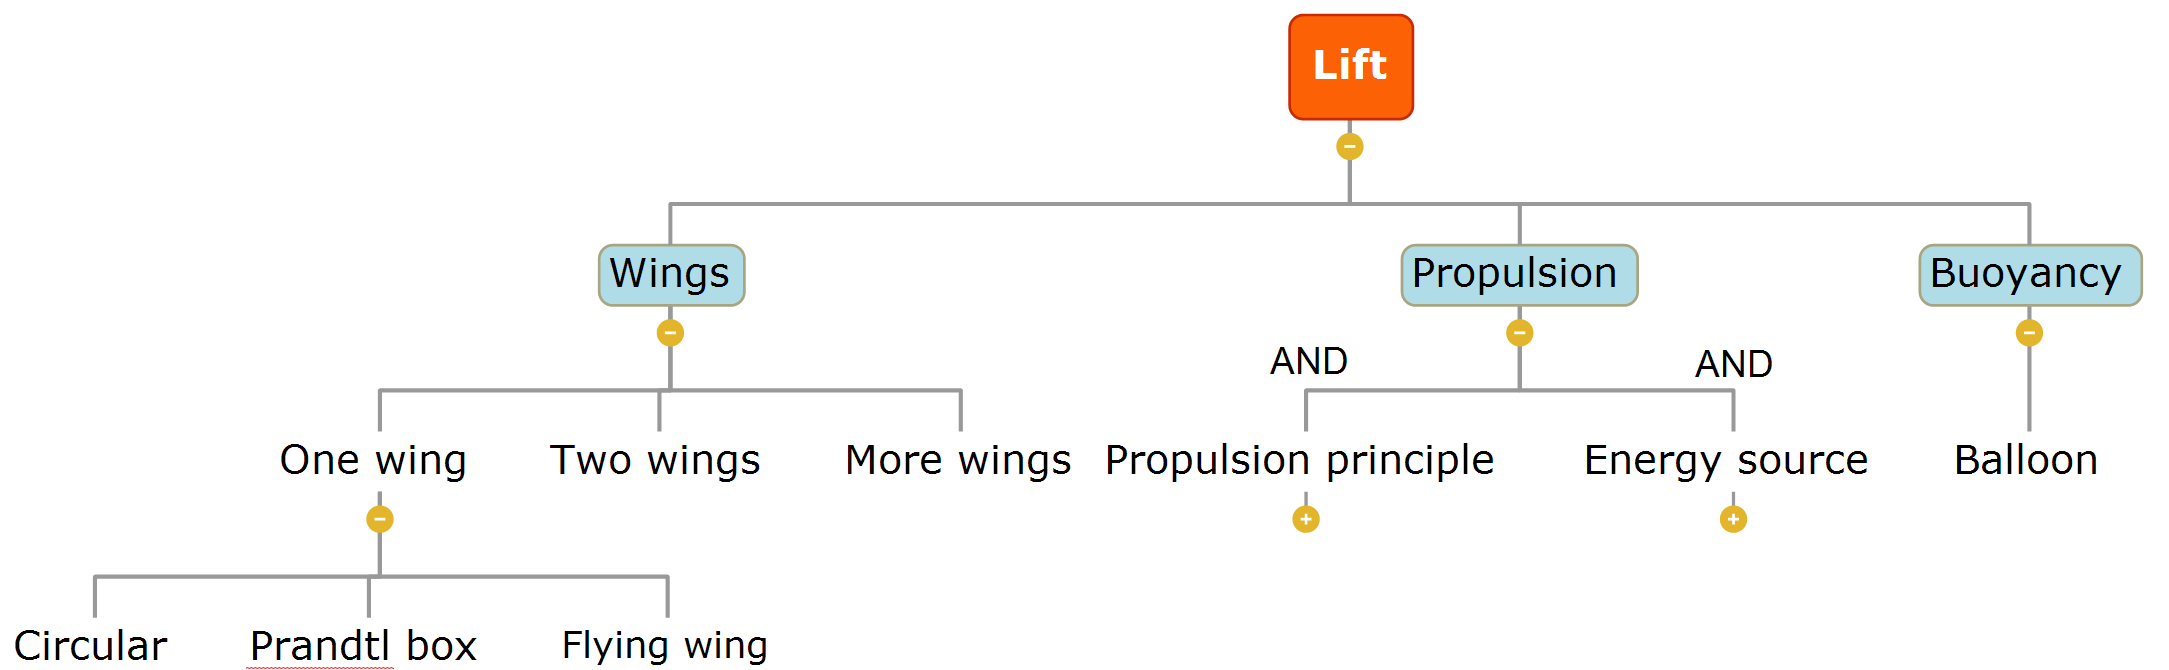
\includegraphics[width=1\textwidth]{Concepts/Figures/Lift}
\caption{Lift branch of the design option tree}
\label{fig:DOTlift}
\end{figure}

\autoref{fig:DOThthrust} shows the choices that there are for the horizontal thrust. When looking at it, it becomes clear that the choices depends on the propulsion, and that there are no other choices. The propulsion AND-tree is shown in \autoref{fig:DOTprop}.

\begin{figure}[H]
\centering
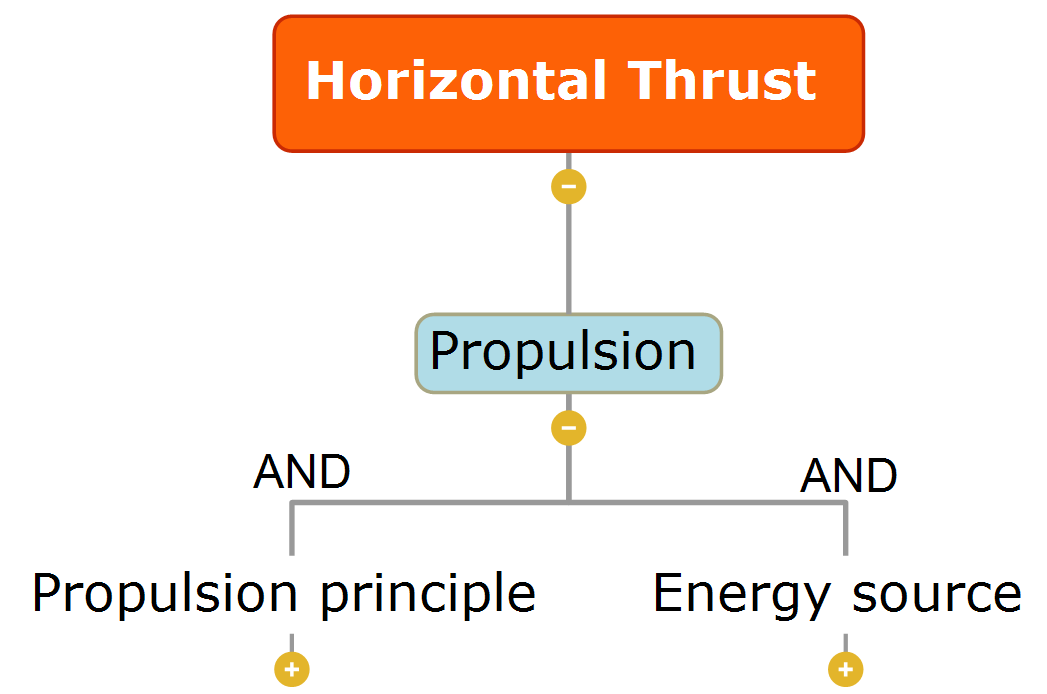
\includegraphics[width=.35\textwidth]{Concepts/Figures/Horizontal_Thrust}
\caption{Horizontal thrust branch of the design option tree}
\label{fig:DOThthrust}
\end{figure}

In \autoref{fig:DOTstability} the stability block of the design option tree is further expanded. It is possible to have active and passive control for this function. The active control can be done with control surfaces or by shifting the mass. For the passive stability the aircraft can make use of an empennage, it can have a dihedral or a sweep for improved stability, or it can use a ballast.

\begin{figure}[H]
\centering
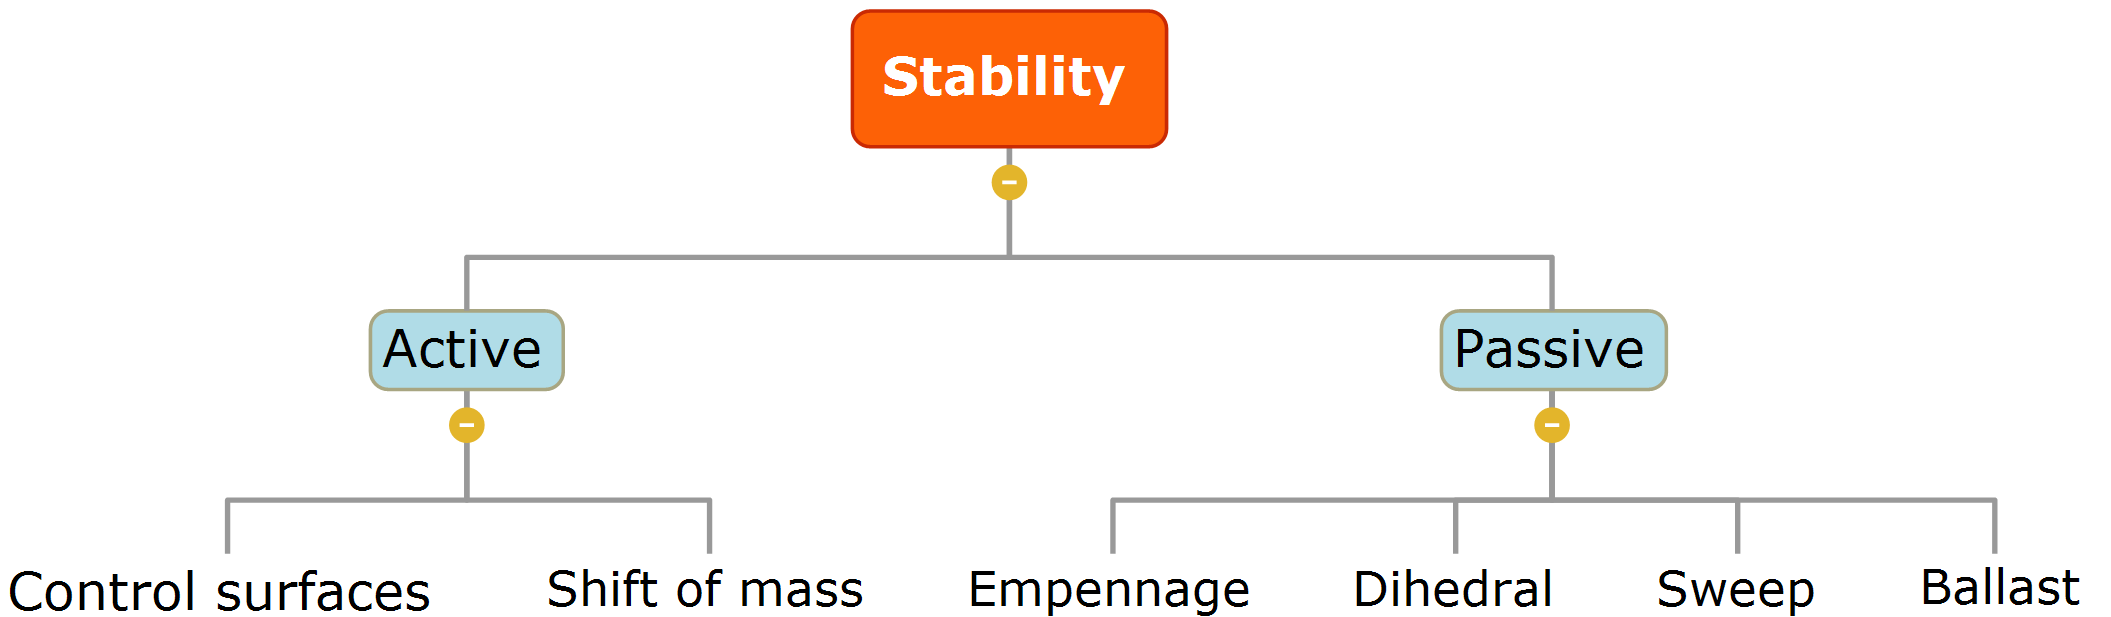
\includegraphics[width=.25\textwidth]{Concepts/Figures/Stability}
\caption{Stability branch of the design option tree}
\label{fig:DOTstability}
\end{figure}

The last function can be seen in \autoref{fig:DOTcontrol}, it depicts how it is possible to control the aircraft. To do this, the aircraft could make use of control surfaces, have morphing wings, shift its mass or make use of plasma air control.

\begin{figure}
    \centering
    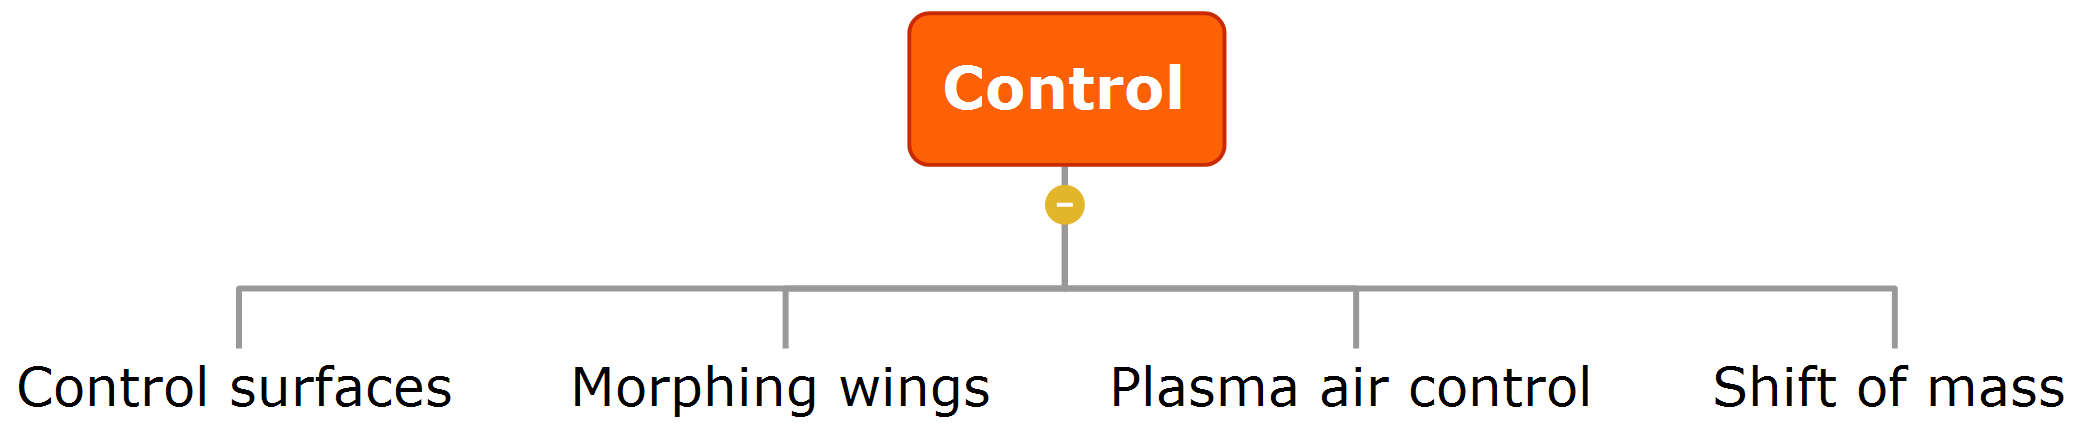
\includegraphics[width=.25\textwidth]{Concepts/Figures/Control}
    \caption{Control Branch of the Design Option Tree}
    \label{fig:DOTcontrol}
\end{figure}

The breakdown of the propulsive options is depicted in \autoref{fig:DOTprop}. The top level propulsion block comprises of both propulsion principle and energy source. The propulsion principle branch on the left side of the tree contains various means of achieving propulsion. On the right side of the tree the energy source branch shows the various methods how to store energy and what kind of energy can be used for propulsion.

\begin{figure}[H]
\centering
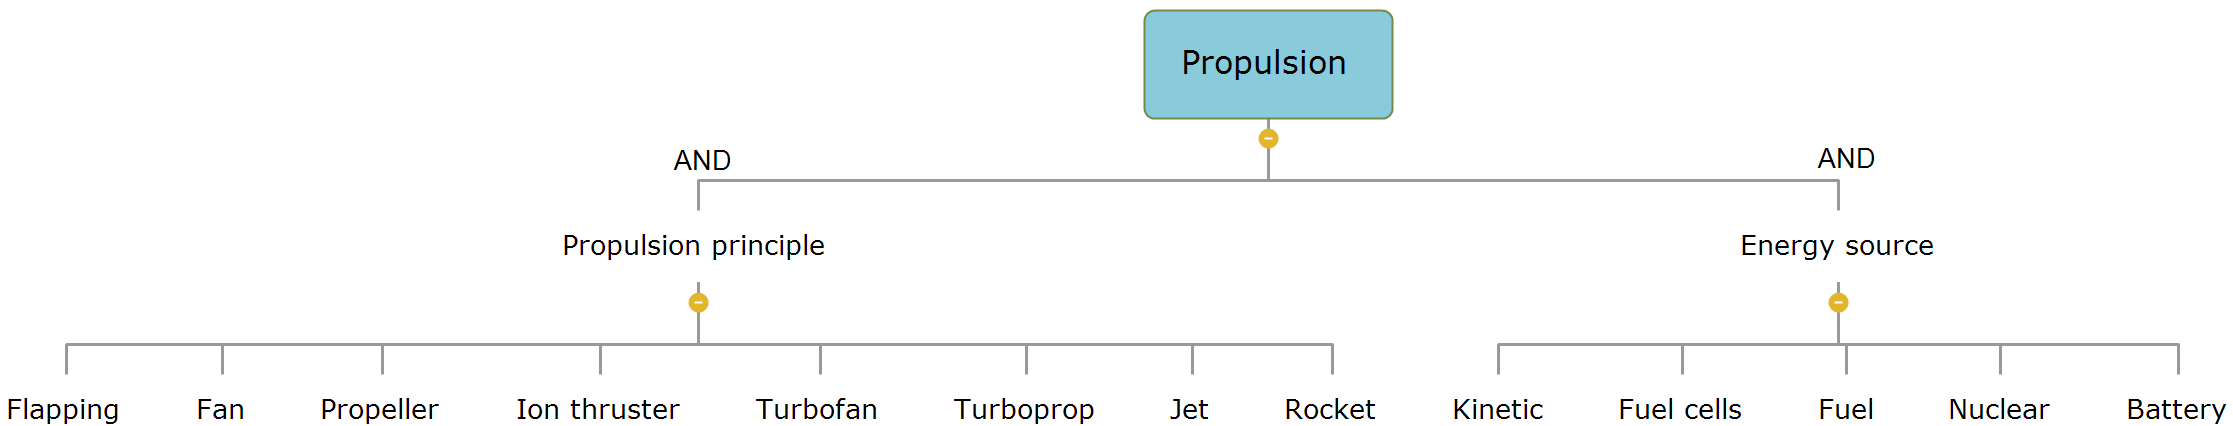
\includegraphics[width=1\textwidth]{Concepts/Figures/Propulsion}
\caption{Propulsion branch of the design option tree}
\label{fig:DOTprop}
\end{figure}

\section{Feasibility Calculations}
\label{sec:feas_calc}
In this section, the airplane-balloon configuration and the Flying Ducted Wing are analysed in a general way to check whether they are feasible concepts or not.

\subsection{Airplane-balloon Configuration}
In order to achieve vertical take-off, landing and hovering for this concept, an inflatable helium balloon is used and needs to generate enough lift. A size of the balloon is estimated based on a simple calculation. A preliminary weight estimation suggests that the UAV weighs 86 kg \cite{baseline}. The density of helium as gas is 0.1664 kg/m$^3$\footnotemark, while that of air is 1.225 kg/m$^3$. Every kilogram of helium can lift 6.3 kg.

%For this concept, the vertical take-off, landing and hovering will be performed using an inflatable helium balloon. In order to do this, the balloon needs to be able to generate enough lift. To check for feasibility, a simple calculation is made. This to estimate the order of the size of the balloon. A preliminary weight estimate of the UAV is 86 kg \cite{baseline}. Since the density of helium, as a gas, is approximately 0.1664 kg/m$^3$\footnotemark, while that of air is approximately 1.225 kg/m$^3$, every kilogram of helium can lift approximately 6.3 kg. 
$$ \frac{1.225}{0.1664} - 1 = 6.3$$

\footnotetext{\url{http://www.engineeringtoolbox.com/gas-density-d_158.html}, Accessed 10-05-2017}


This means 14 kg of Helium is needed to lift the UAV. It requires a balloon of 85 m$^3$, equivalent to 85000 litres. Because of the unrealistic size of the balloon, the balloon concept is deemed infeasible and therefore removed from further development.

\subsection{Flying Ducted Wing}
The flying ducted wing concept has integrated ducts that deflect the exhaust air downward, in order to generate vertical forces. These can be used to perform vertical take-off and landing, as well as hovering. The feasibility of this concept is tested by a very general calculation in which the required downward exhaust velocity is estimated. It is assumed the outlet diameter equals 15 cm, based on the payload. In the case of four ducts, the outlet flow velocity should be in the order of 100 m/s. As the horizontal velocity is zero when taking off, the air should be accelerated from 0 to more than 100 m/s as it will slow down after going through the duct. Therefore, this concept is deemed infeasible.
$$F = \dot{m} v = \rho A v^2 $$
$$v^2 = \frac{F}{4 \cdot \rho A} = \frac{9.81 \cdot 86}{4 \cdot 1.225 \cdot 0.15^2 \cdot \frac{\pi}{4}}$$

\nomenclature[G]{$\rho$}{Density \nomunit{kg/m$^3$}}

\section{Chosen Concepts}
\label{sec:chosconc}

Based on the above calculations, both the airplane-balloon configuration as well as the flying ducted wing will not be analysed any further. It is decided to continue with the remaining three concepts. In order to make sure that enough concepts are compared, two extra concepts are added. These are a tailsitter and a UAV that is a combination of a quadcopter and a conventional aircraft. A summary of each concept is given in this section. Since the manner in which the payload is mounted has not been discussed for the concepts, it will also be elaborated in this section. Different concepts make use of different payload mounting methods, but they all have in common that they enable monitoring equipment to be placed at the bottom of the UAVs and it is possible to release the payload while hovering. 

\begin{comment}
- Door in the fuselage at the end
- Opening on bottom of FL
- click mechanism closed or open
- Removable payload section as part of fuselage
\end{comment}

\subsection{Concept \#1: The Tailsitter}
The Tailsitter can be seen in \autoref{fig:tail_conc}. It does not have movable wings of propellers. Instead, the entire UAV rotates when transitioning from vertical to horizontal flight. Since this is a proven concept\footnotemark, no extra calculations are made before performing the technical analysis. 

In terms of payload mounting, The Tailsitter poses the most difficulty using the payload for monitoring operations. This is because while hovering, the payload area facing downward is 15 x 15 cm instead of 15 x 100 cm as is the case for the other concepts. Therefore, the recording part of the monitoring payload can not be as large in this design as it could in others. The payload will be loaded through the tail. Any payload module should have the same end, that can click into the back. The UAV can then simply release the module and drop it to a designated area.

\footnotetext{\url{http://www.atmosuav.com/}, Accessed 09-05-2017}


\begin{figure}[htb]
\centering
\begin{minipage}{.5\textwidth}
  \centering
  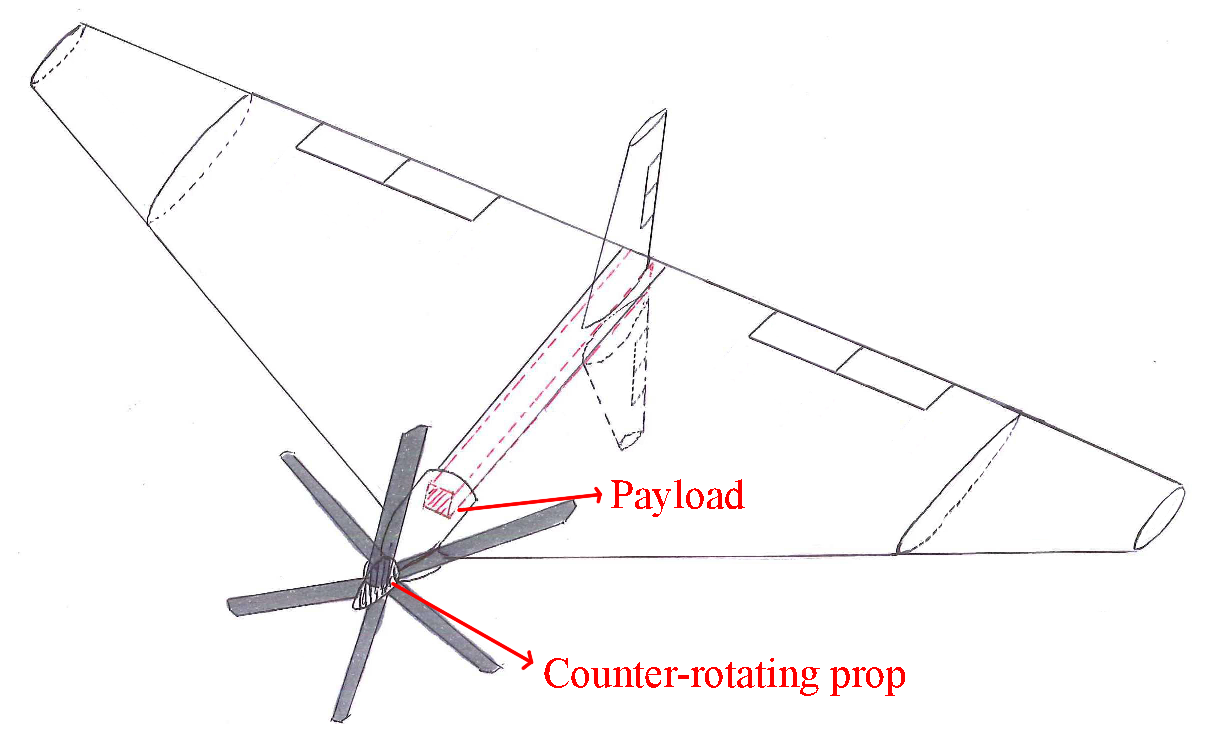
\includegraphics[width=.95\linewidth]{Concepts/Figures/Tailsitter}
  \captionof{figure}{Concept 1: The Tailsitter}
  \label{fig:tail_conc}
\end{minipage}%
\begin{minipage}{.5\textwidth}
  \centering
  \includegraphics[width=.95\linewidth]{Concepts/Figures/Tandem}
  \captionof{figure}{Concept 2: The Tandem}
  \label{fig:tand_conc}
\end{minipage}
\end{figure}


\subsection{Concept \#2: The Tandem}
The tandem concept was already explained in the baseline report \cite{baseline}. It consists of a tandem wing configuration where the wings can be rotated. The layout of the concept can be seen in \autoref{fig:tand_conc}. The feasibility of this concept has been proven\footnotemark.
\footnotetext{\url{http://www.airbusgroup.com/int/en/news-media/media~item=f2c37ffd-dbe4-41c0-b017-ba8ca60bce25~.html}, Accessed 10-05-2017}

The payload can be loaded and unloaded through the back of the fuselage section, where a 'door' is present. In case monitoring equipment is required, the fuselage should contain see-through sections at the bottom. 


\subsection{Concept \#3: The Prandtl Box}
%all that needs to be done is to insert the sketch! name it Prandtl Box
The Prandtl Box analysed in this report has been altered slightly from the concept presented in the baseline report\cite{baseline}. It is done because integrating the propellers in the wing sets a limit on the size of the blades. In the altered concepts, the wing configuration is the same, but the propulsion system is placed in a different location. In the altered setup, this concept has been proven to be feasible\footnotemark. The updated concept can be seen in \autoref{fig:pran_box_conc}
\footnotetext{\url{http://www.avy.eu}, Accessed 10-05-2017}.

The payload will be loaded using a door-like device on the bottom of the UAV. This allows for easy unloading while hovering.

\begin{figure}[htb]
\centering
\begin{minipage}{.5\textwidth}
    \centering
    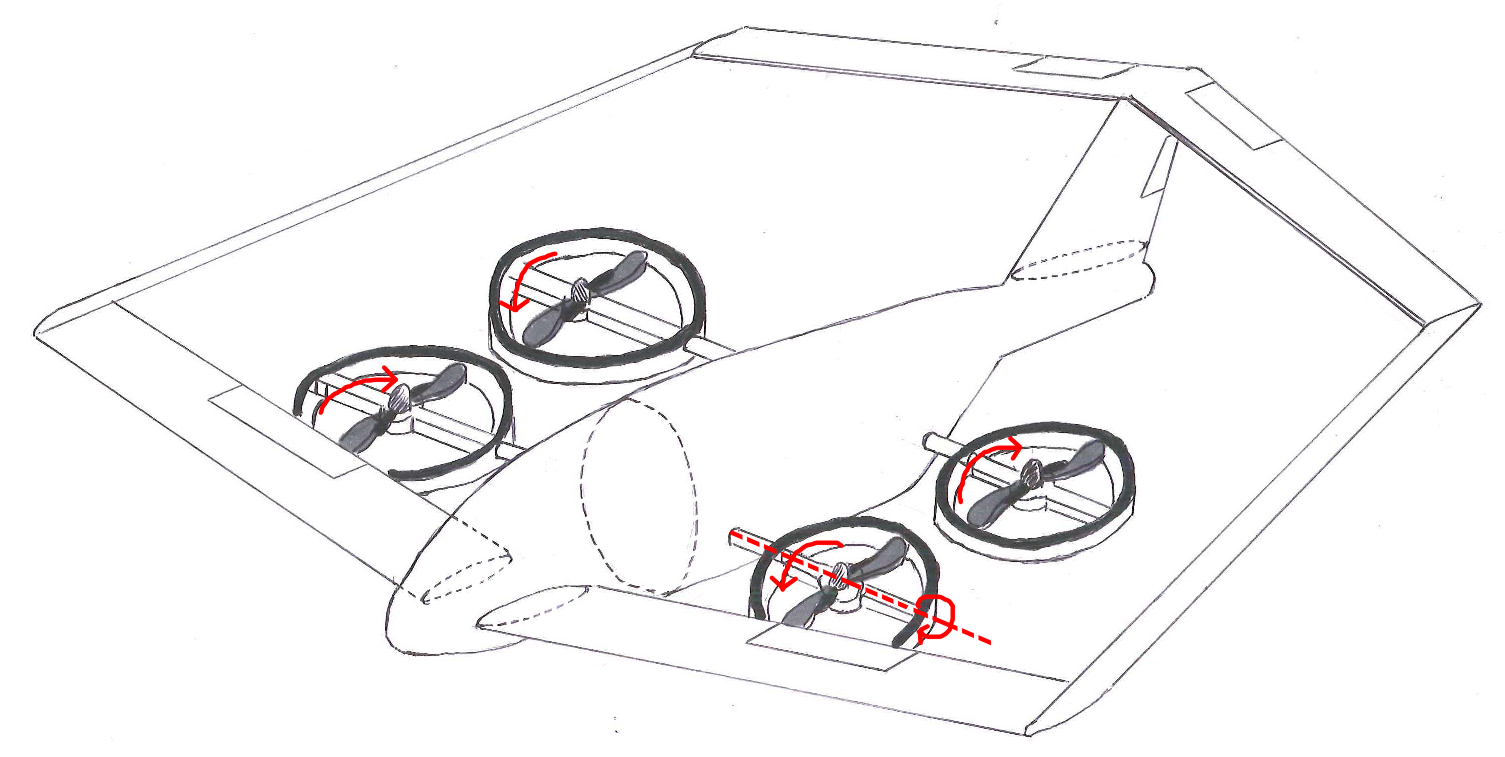
\includegraphics[width = .95\linewidth]{Concepts/Figures/PrandtlBox}
    \captionof{figure}{Concept 3: The Prandtl Box}
    \label{fig:pran_box_conc}
\end{minipage}
\begin{minipage}{.49\textwidth}
    \centering
    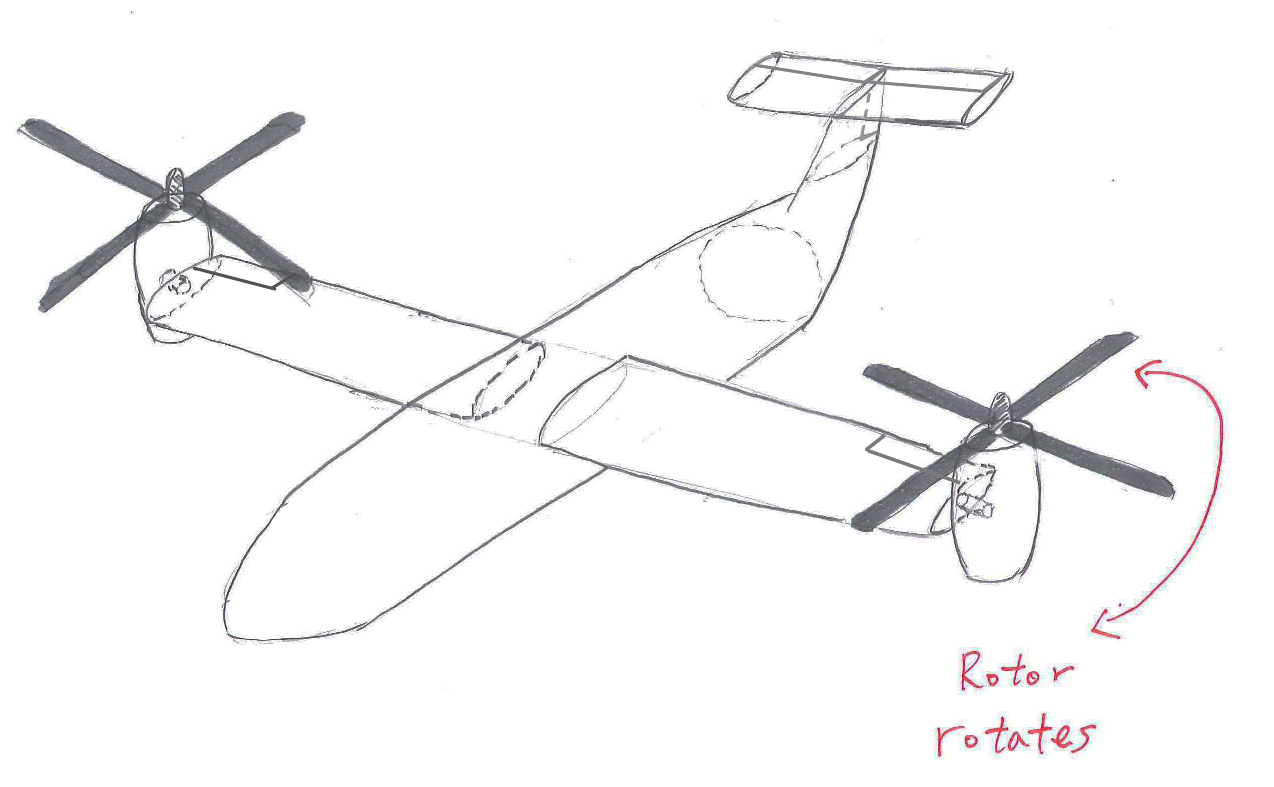
\includegraphics[width=.95\linewidth]{Concepts/Figures/TiltRotor}
    \captionof{figure}{Concept 4: The Tiltrotor}
    \label{fig:tilt_roto_conc}    
\end{minipage}
\end{figure}




\subsection{Concept \#4: The Tiltrotor}
The Tiltrotor is already explained in the baseline report \cite{baseline}. It consists of a fuselage with a wing, where the rotors are attached at the tip of the wing. It is possible to rotate the rotors for horizontal and vertical propulsion. The Tiltrotor can be seen in \autoref{fig:tilt_roto_conc}

The payload will be mounted using a separate payload module that is mounted to the fuselage using a clicking device. The entire payload module can exit the aircraft.




\subsection{Concept \#5: The Winged Quadcopter}
Based on a team discussion, it is decided that a working hybrid UAV design should be included in the analysis. Thus, a winged quadcopter configuration\footnote{\url{https://latitudeengineering.com/products/hq/}, Accessed 10-05-2017} is chosen for analysis. The design can be seen in \autoref{fig:wing_quad_conc}.

% Since two unfeasible concepts were eliminated, time is available to analyse another concept. It was decided that a winged quadcopter configuration will be analysed, because it is one of the most frequently used layouts for hybrid UAVs\footnote{\url{https://latitudeengineering.com/products/hq/}, Accessed 10-05-2017}. The suggested layout can be seen in \autoref{fig:wing_quad_conc}

\begin{figure}[htb]
    \centering
    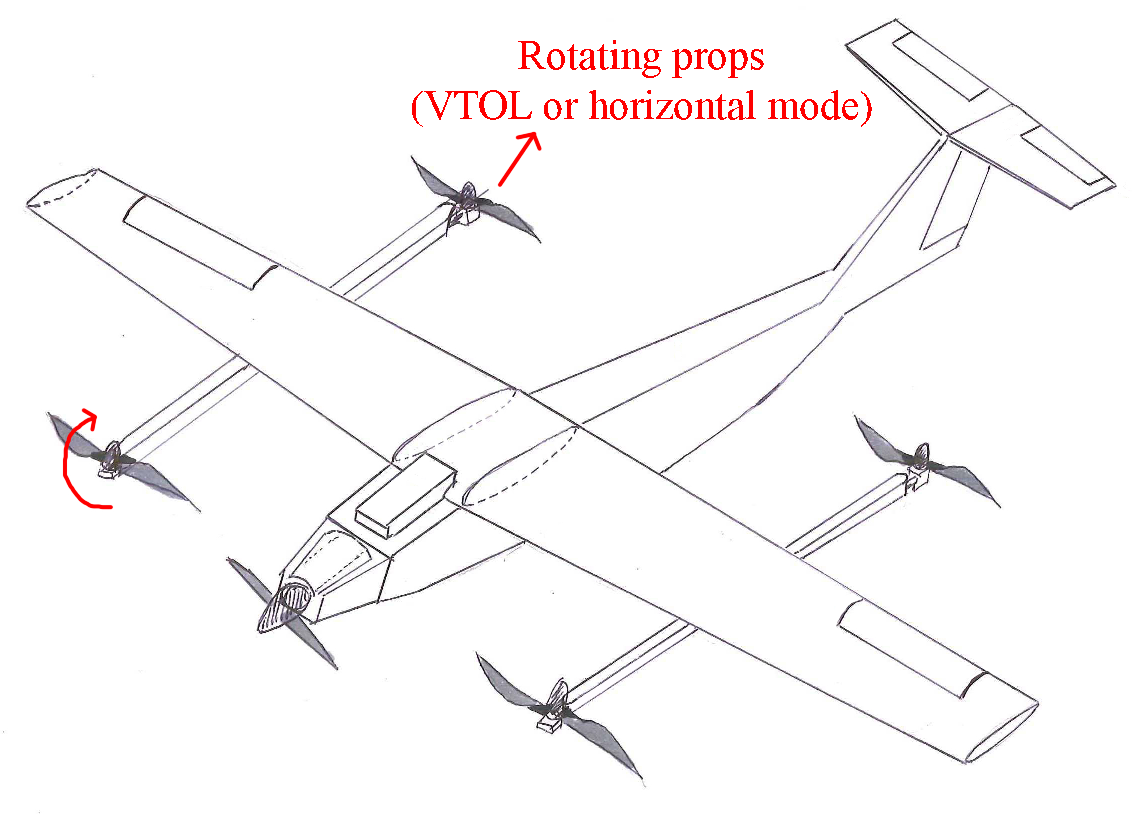
\includegraphics[width=.475\textwidth]{Concepts/Figures/WingedQuadcopter}
    \caption{Concept 5: Winged Quadcopter}
    \label{fig:wing_quad_conc}
\end{figure}

The payload will be mounted similar to the one in The Tiltrotor using a separate payload module that can be replaced and clicked into the fuselage.